\documentclass{../../ece-report}

\usepackage{subcaption}
\usepackage{multirow}


\memostudent{Ty Davis}
\memotitle{Lab 6 - Common Source Amplifier using NMOS Transistor}
\memocourse{ECE 3110}
\memodate{\today}


\newcommand{\Vsub}[1]{\ensuremath{\textnormal{V}_{#1}}}
\newcommand{\sub}[2]{\ensuremath{\textnormal{#1}_{#2}}}

\renewcommand{\half}{\frac{1}{2}}



\begin{document}

\maketitle


\section{Introduction and Theory}


The circuit that we are analyzing in this lab is shown
in Fig.~\ref{fig:circuit_full}. This circuit is an NMOS
based common source amplifier, and we are going to design
the circuit such that the gain is $A_v = -10~\si{\V/\V}$.
We know that  $R_L = 10~\si{\kohm}$, $R_G = 10~\si{\kohm}$,
and $R_\textnormal{sig} = 50~\si{\ohm}$, and we want
the circuit to have $I_D = 1~\si{\mA}$. As such, we will need 
to select the resistors $R_S$ and $R_D$ that meet these conditions.
In order to do this, we are going to analyze the circuit
in both DC and AC situations.

\begin{figure}[h!]
  \centering
    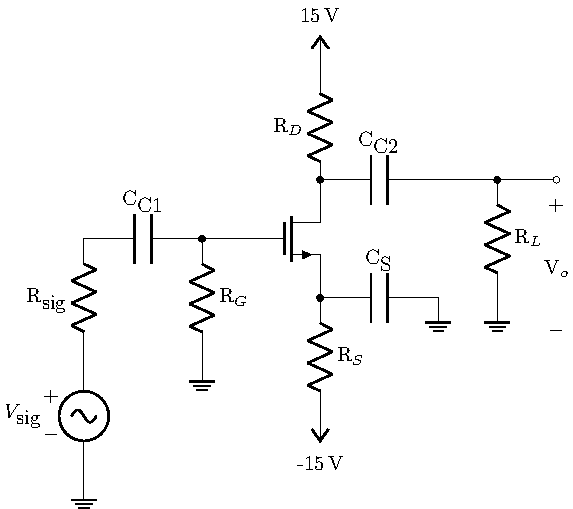
\includegraphics{../circuits/circuit_full.pdf}
  \caption{The circuit that we are analyzing in this lab.}\label{fig:circuit_full}
\end{figure}


\section{DC Analysis}

\begin{figure}[h!]
  \centering
  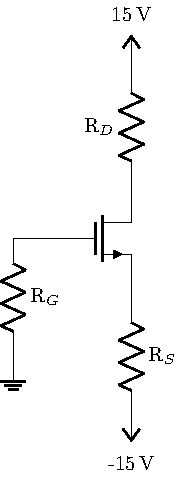
\includegraphics{../circuits/circuit_dc.pdf}
  \caption{The circuit reduced for DC analysis.}\label{fig:circuit_dc}
\end{figure}

In Fig.~\ref{fig:circuit_dc} we can see how the circuit
behaves when the considering the DC analysis. Because
the capacitors act as open circuits in DC, the circuit
is significantly reduced. The DC current through $R_G$ is 0~A.

Using the expression

\[
  V_{GS} = \sqrt{ \frac{2 I_D}{k_n}} + V_{th}
\]

we can determine that the voltage $V_{GS}$ is $V_{GS}= 2.269~\si{\V}$.

This yields $V_{ov}= V_{GS} - V_{th} = 0.169~\si{\V}$.

Also, because $V_G$ is 0~V, we know that $V_S = -V_{GS}
= -2.269~\si{\V}$. Using that value for $V_S$ we can find that $R_S = 12.731~\si{\kohm}$.

Finishing off the DC analysis we know from the Early voltage that
$r_0 = 4165~\si{\V} / 1~\si{\mA} = 4.17~\si{\Mohm}$.

\section{AC Analysis}

\begin{figure}[h!]
  \centering
  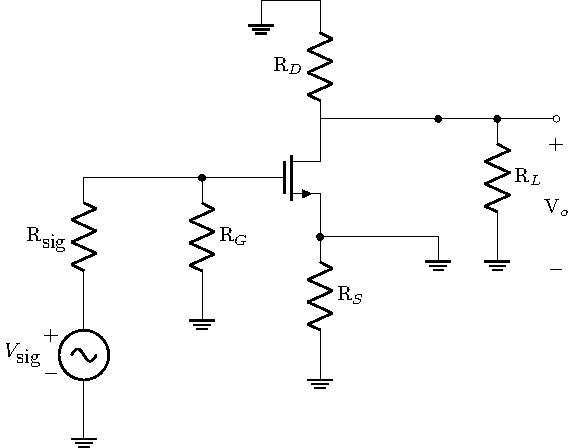
\includegraphics{../circuits/circuit_ac.pdf}
  \caption{The circuit reduced for AC analysis.}\label{fig:circuit_ac}
\end{figure}

In AC analysis, the sufficiently large capacitors can be replaced
with shorts, and the circuit that remains is shown in Fig.~\ref{fig:circuit_ac}.

Note as well that the resistor $R_S$ is shorted to ground on both sides
and therefore doesn't have an affect on the circuit either. As such
the voltage $V_S = 0~$V.

When using the hybrid-$\pi$ model, we can determine that the voltage $V_o = V_D (r_0 \| R_L)$.
This is essentially the same as the expression $A_v = -g_m (R_0 \| R_D)$. 

Knowing that $g_m = k_n / V_{ov}$, and $A_v = 10$, we can find that $R_D = 841 \si{\ohm}$.

This concludes the analysis that we need to do on the circuit, now we can simulate
and measure the performance of the circuit.

\section{Simulation}

When simulating the circuit with Multisim, we found that the gain of the circuit
was 9.88~\si{\V/\V}. This is right what we expected from our analysis.
You can see the results of the simulation in Fig.~\ref{fig:sim}.

\begin{figure}[h!]
  \centering
  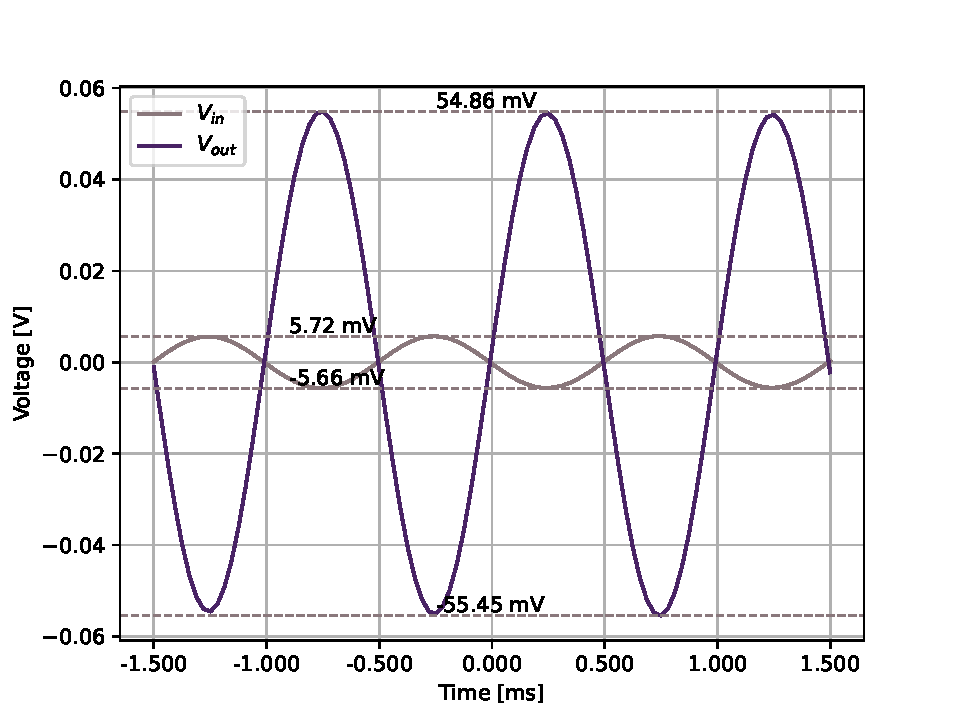
\includegraphics[width=0.6\textwidth]{../plots/pdf/sim.pdf}
  \caption{Simulated Circuit Output.}\label{fig:sim}
\end{figure}



\section{Results}

When the circuit is built and measured, we find that
the value for $A_v$ is $A_v = 6.67 \si{\V/\V}$. This
is just a little low, so we increase the resistor $R_D$
until we get about what we want for the gain. We found
that using a resistor $R_D \approx 1340 \si{\ohm}$ yielded
about $A_v = 9.46 \si{\V/\V}$ which was just what we
wanted. You can see these results in Fig.~\ref{fig:gain6_67}
and Fig.~\ref{fig:gain9_47}.



\begin{figure}[h!]
  \centering
  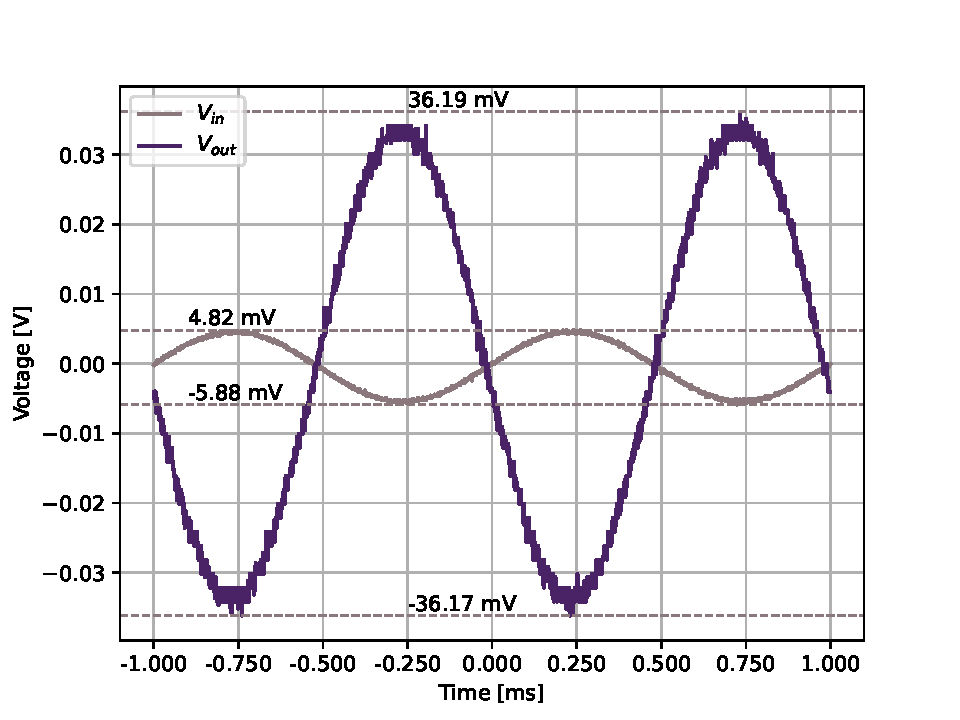
\includegraphics[width=0.6\textwidth]{../plots/pdf/gain6_67.pdf}
  \caption{Circuit with 841 \si{\ohm}. Gain is $A_v=6.67$.}\label{fig:gain6_67}
\end{figure}

\begin{figure}[h!]
  \centering
  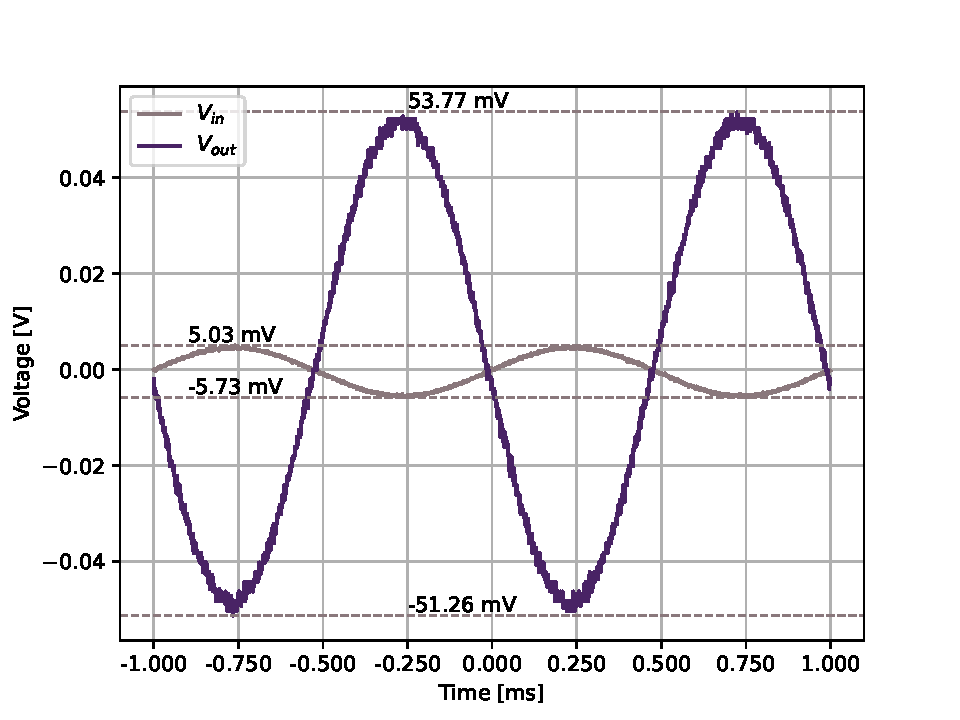
\includegraphics[width=0.6\textwidth]{../plots/pdf/gain9_46.pdf}
  \caption{Circuit with 1341 \si{\ohm}. Gain is $A_v=9.46$.}\label{fig:gain9_47}
\end{figure}

When placing a 1 \si{\Mohm} resistor for $R_L$ we found the gain to be about 8,
and the gain was halved with $R_L$ was all the way down to just $R_L = 470~\si{\ohm}$.

\begin{figure}[h!]
  \centering
  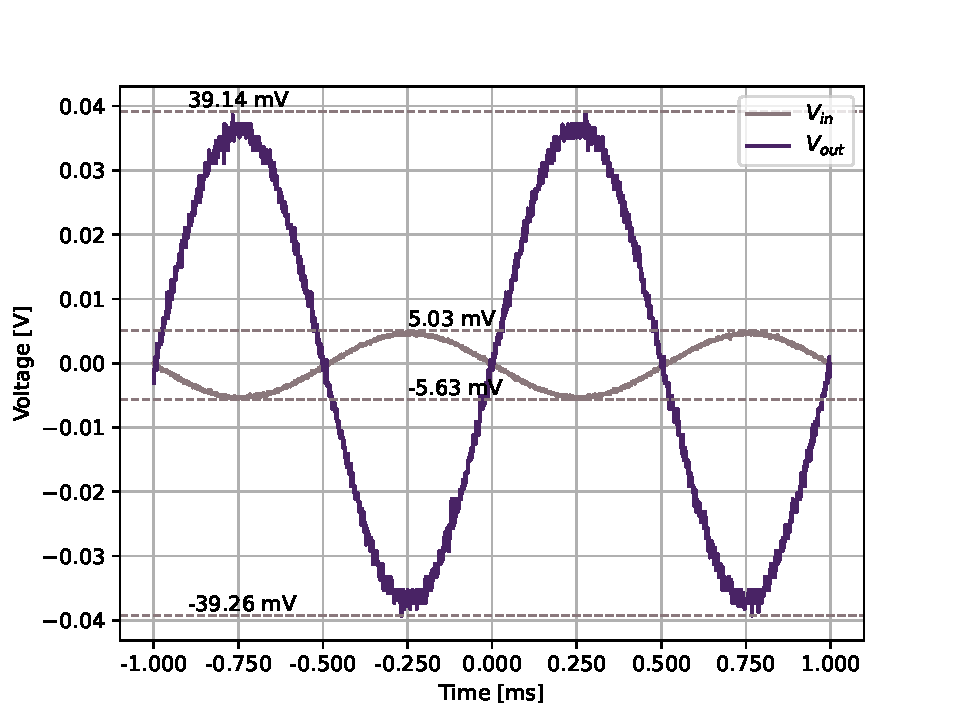
\includegraphics[width=0.6\textwidth]{../plots/pdf/rl_1meg.pdf}
  \caption{Circuit with 1 \si{\Mohm}. Gain is $A_v=8$}\label{fig:1meg}
\end{figure}

\begin{figure}[h!]
  \centering
  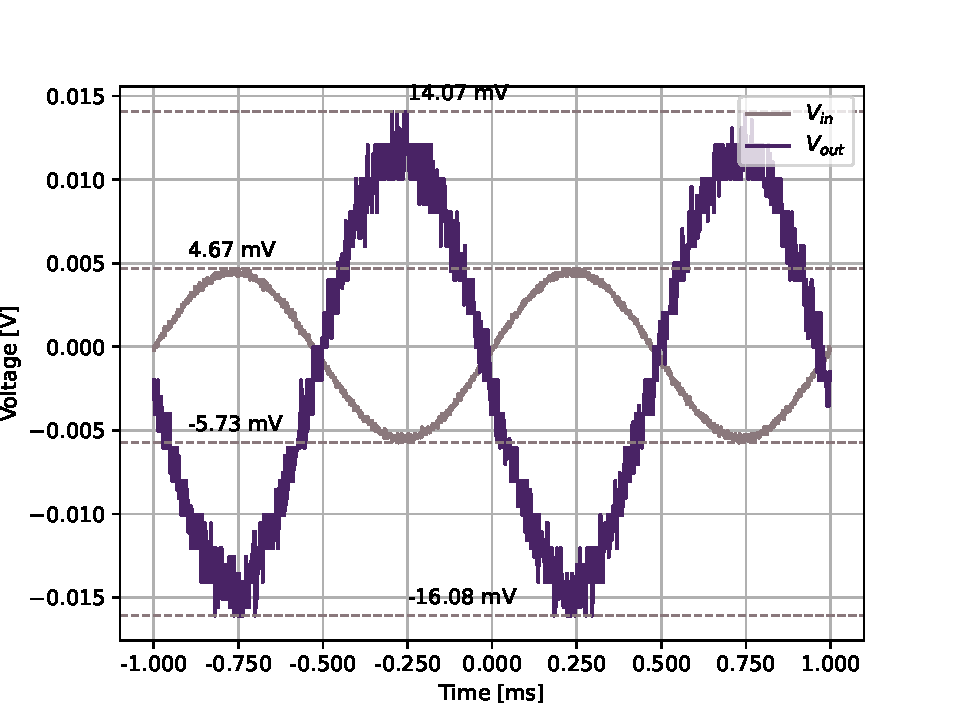
\includegraphics[width=0.6\textwidth]{../plots/pdf/rl_470.pdf}
  \caption{Circuit with 470 \si{\ohm}. Gain is half of when $R_L=1~\si{\Mohm}$.}\label{fig:470ohm}
\end{figure}

\begin{figure}[h!]
  \centering
  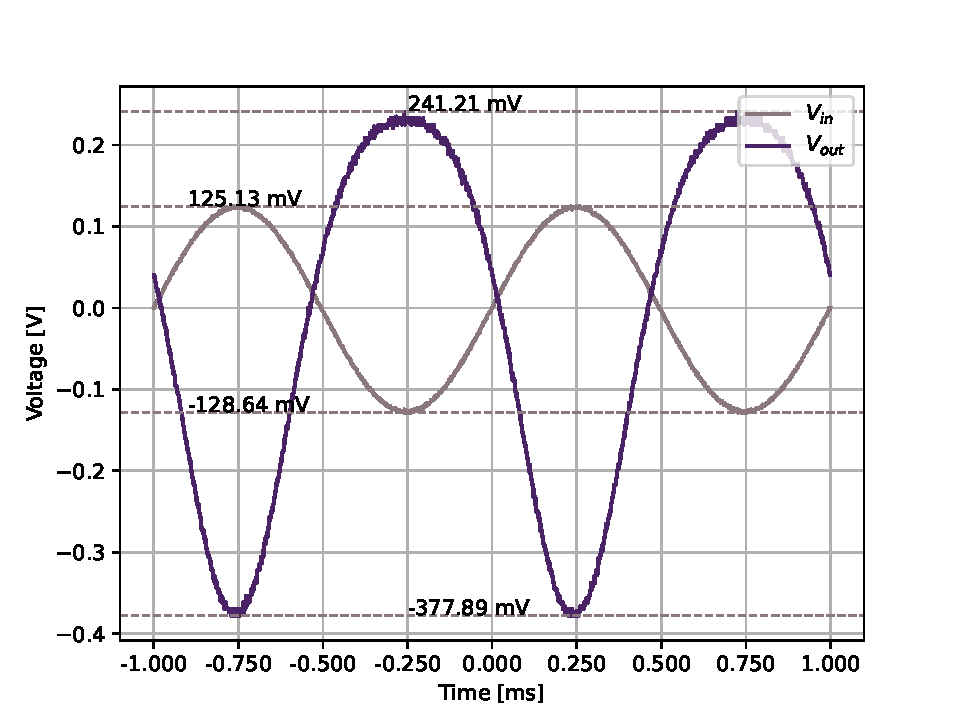
\includegraphics[width=0.6\textwidth]{../plots/pdf/vi_250m.pdf}
  \caption{Circuit with input voltage $V_\textnormal{sig} ~\approx$ 250~\si{\mV}.}\label{fig:250m}
\end{figure}

\begin{figure}[h!]
  \centering
  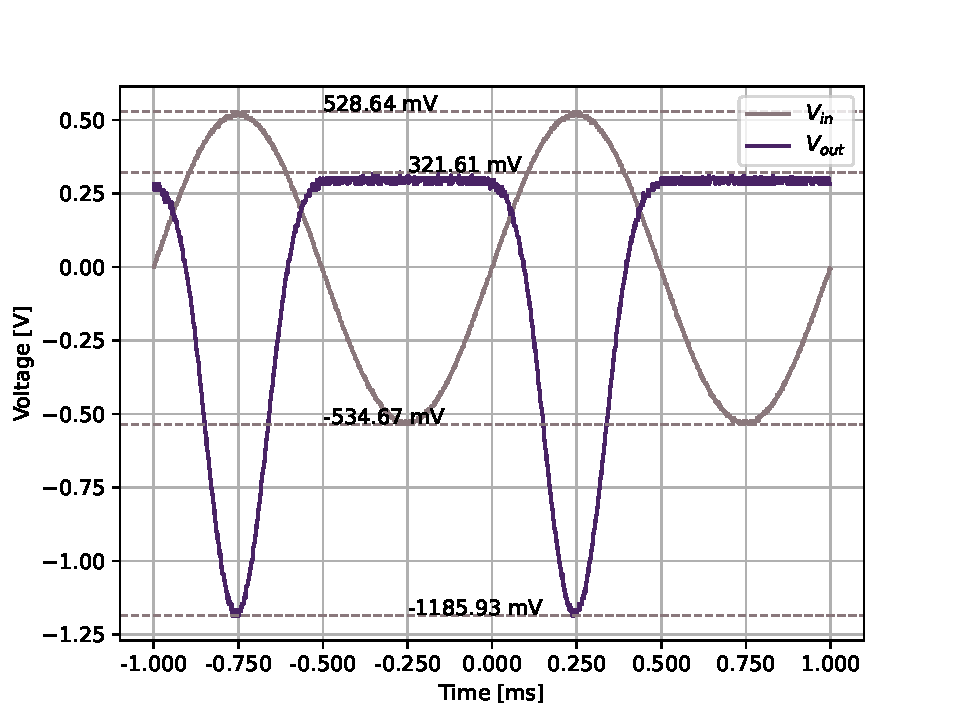
\includegraphics[width=0.6\textwidth]{../plots/pdf/vi_1v.pdf}
  \caption{Circuit with input voltage $V_\textnormal{sig} ~\approx$ 1~\si{\V}.}\label{fig:1V}
\end{figure}




Table~\ref{tab:resistors} shows the values that were
calculated, found equivalently and measured in the experimental
portion of the lab.

\begin{table}[h!]
  \centering
  \begin{tabular}{l l l c}\toprule
    \textbf{Calculated Resistor} & \textbf{Equivalent Resistor} & \textbf{Measured Resistor} & \\
    \midrule

12.731 \si{\kohm} & 12.691 \si{\kohm} & 12.529 \si{\kohm} & $R_S$ \\
          & 100 \si{\kohm}    & 99.0 \si{\kohm}   &       \\
          & 15 \si{\kohm}     & 14.80 \si{\kohm}  &       \\
          & 470 \si{\kohm}    & 464.8 \si{\kohm}  &       \\
          \midrule
841 \si{\ohm}    & 840 \si{\ohm}    & 831 \si{\ohm}    & $R_D$ \\
          & 10 \si{\ohm}     & 9.93 \si{\ohm}   &       \\
          & 150 \si{\ohm}    & 148.6 \si{\ohm}  &       \\
          & 680 \si{\ohm}    & 673.4 \si{\ohm}  &       \\
(1341 \si{\ohm})   & (470 \si{\ohm})  & (464 \si{\ohm})  &       \\
          \midrule
10 \si{\kohm}     & 10 \si{\kohm}     & 9.893 \si{\kohm}  & $R_G$ \\
          \midrule
10 \si{\kohm}     & 10 \si{\kohm}     & 9.837 \si{\kohm}  & $R_L$ \\
(1 \si{\Mohm})      & (1 \si{\Mohm})      & (970 \si{\kohm})    &      \\
\bottomrule
\end{tabular}
\caption{Measured resistors.}
\label{tab:resistors}
\end{table}

The output voltage started to rail when the input voltage
was increased. There was some distortion around $V_\textnormal{sig}
= 250~\si{\mV}$, and extreme distortion as high as $V_\textnormal{sig}
= 1~\si{\V}$. This is demonstrated in Figs.~\ref{fig:250m} and \ref{fig:1V}.

\section{Conclusion/Post Lab Observations}

The driving resistor was the lowest resistor between $R_0$, $R_D$, and $R_L$ because 
of their parallel configuration. The circuit demonstrated that the NMOS transistor
can be used as an amplifier, but the output resistance can have an affect on the amplification
when below the value for $R_D$.

With an increasingly high input voltage, the output voltage began to rail, as you can see in Figs.~\ref{fig:250m} and \ref{fig:1V}.

\end{document}
